% 
% Copyright 2019-2020 Elsevier Ltd
% 
% This file is part of the 'CAS Bundle'.
% --------------------------------------
% 
% It may be distributed under the conditions of the LaTeX Project Public
% License, either version 1.2 of this license or (at your option) any
% later version.  The latest version of this license is in
%    http://www.latex-project.org/lppl.txt
% and version 1.2 or later is part of all distributions of LaTeX
% version 1999/12/01 or later.
% 
% The list of all files belonging to the 'CAS Bundle' is
% given in the file `manifest.txt'.
% 
% Template article for cas-dc documentclass for 
% double column output.

%\documentclass[a4paper,fleqn,longmktitle]{cas-dc}
\documentclass[a4paper,fleqn]{cas-dc}

%\usepackage[numbers]{natbib}
\usepackage[authoryear]{natbib}
\usepackage{amsmath}
\usepackage{tabularx}
%\usepackage[authoryear,longnamesfirst]{natbib}
\usepackage{blindtext}
\usepackage{graphicx}
%%%Author definitions
\def\tsc#1{\csdef{#1}{\textsc{\lowercase{#1}}\xspace}}
\tsc{WGM}
\tsc{QE}
\tsc{EP}
\tsc{PMS}
\tsc{BEC}
\tsc{DE}
%%%

% Uncomment and use as if needed
%\newtheorem{theorem}{Theorem}
%\newtheorem{lemma}[theorem]{Lemma}
%\newdefinition{rmk}{Remark}
%\newproof{pf}{Proof}
%\newproof{pot}{Proof of Theorem \ref{thm}}

\begin{document}
\let\WriteBookmarks\relax
\def\floatpagepagefraction{1}
\def\textpagefraction{.001}

% Research highlights
\begin{highlights}
\item Research highlights item 1
\item Research highlights item 2
\item Research highlights item 3
\end{highlights}

% Short title
\shorttitle{
Assessing the Drought State Transition in a human-modified basin
}

% Short author
\shortauthors{Carlos E. S. Lima \textit{et~al}.}

% Main title of the paper
\title [mode = title]{
Assessing the Drought State Transition in a human-modified basin
}                      
%Declaração dos autores!
% First author
%
% Options: Use if required
% eg: \author[1,3]{Author Name}[type=editor,
%       style=chinese,
%       auid=000,
%       bioid=1,
%       prefix=Sir,
%       orcid=0000-0000-0000-0000,
%       facebook=<facebook id>,
%       twitter=<twitter id>,
%       linkedin=<linkedin id>,
%       gplus=<gplus id>]

\author[1]{Carlos E. S. Lima}[type=editor,
                        %auid=000,bioid=1,
                        orcid=0000-0001-7511-2910]
\cormark[1]
% Footnote of the first author
%\fnmark[1]
\ead{eduardolima@alu.ufc.br}
\credit{Data curation, Writing - Original draft preparation}

% Second author
\author[1]{Marx V. M. da Silva}[orcid=0000-0001-7511-2910]
\credit{Data curation, Writing - Original draft preparation}
\ead{marx.silva@alu.ufc.br}
% Third author
\author[1]{Sabrina S. Monteiro}[orcid=0000-0001-7511-2910]
\credit{Data curation, Writing - Original draft preparation}
\ead{sabrina.monteiro00@alu.ufc.br }

% Fourth author
\author[1]{Cleiton S. Silveira}[orcid=0000-0001-7511-2910]
\ead{cleitonsilveira@ufc.br }
\credit{Data curation, Writing - Original draft preparation}

%  Credit authorship
\credit{Conceptualization of this study, Methodology, Software}

% Address/affiliation
\affiliation[1]{organization={
    Dept. of Hydraulic and Environmental Engineering (DEHA), Federal University of Ceará (UFC)},
    %addressline={Radarweg 29}, 
    city={Fortaleza},
    % citysep={}, % Uncomment if no comma needed between city and postcode
    postcode={60440-970}, 
    state={CE},
    country={Brazil}}


% Title footnote mark
% eg: \tnotemark[1]
%\tnotemark[1,2]

% Title footnote 1.
% eg: \tnotetext[1]{Title footnote text}
% \tnotetext[<tnote number>]{<tnote text>} 
%\tnotetext[1]{This document is the results of the research
   %project funded by the National Science Foundation.}

%\tnotetext[2]{The second title footnote which is a longer text matter
   %to fill through the whole text width and overflow into
   %another line in the footnotes area of the first page.}

% For a title note without a number/mark
%\nonumnote{This note has no numbers. In this work we demonstrate %$a_b$
  %the formation Y\_1 of a new type of polariton on the interface
  %between a cuprous oxide slab and a polystyrene micro-sphere placed
  %on the slab.
  %}

% Corresponding author text
\cortext[cor1]{Corresponding author}
%\cortext[cor2]{Principal corresponding author}

% Footnote text
%\fntext[fn1]{This is the first author footnote. but is common to %third
  %author as well.}
%\fntext[fn2]{Another author footnote, this is a very long footnote and
  %it should be a really long footnote. But this footnote is not yet
  %sufficiently long enough to make two lines of footnote text.}


% Here goes the abstract
\begin{abstract}
In the Anthropocene, human activities began to exert a great influence on the planet's natural cycles. In relation to droughts, anthropic activities have become an increasingly representative component in the processes of generation and development of this phenomenon. In this context, methodologies capable of identifying signs of anthropic impacts on the aforementioned processes become of utmost importance for efficient drought management. In the present study, it was sought to evaluate the changes in the transition patterns between meteorological and hydrological drought classes and in the probability of occurrence of these drought classes for a sub-basin of the São Francisco River Hydrographic Basin (BHSF), more precisely in western Bahia, for two reference periods: P1, from 1935 to 1984, and P2, from 1985 to 2020. The Standard Precipitation Index (SPI) and Standard Runoff Index (SRI) drought indices were adopted to characterize meteorological and hydrological droughts, respectively. The transition analysis between drought classes and their occurrence probabilities was performed using Markov Chains, considering the SPI and SRI series in periods P1 and P2. The results pointed to a higher probability of occurrence of hydrological and meteorological droughts classified as Severe or Extreme in the P2 period, with a higher probability of persistence of this state in hydrological droughts. The meteorological droughts, in its turn, showed no possibility of persistence of this state, suggesting that the persistence observed in hydrological droughts may be associated with mechanisms other than precipitation.
\end{abstract}

% Use if graphical abstract is present
% \begin{graphicalabstract}
% 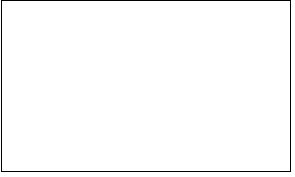
\includegraphics{figs/grabs.pdf}
% \end{graphicalabstract}


% Keywords
% Each keyword is seperated by \sep
\begin{keywords}
Drought Transition \sep Markov Chain \sep Anthropic Changes \sep Minimum Streamflow
\end{keywords}


\maketitle

\section{Introduction}
	As secas são fenômenos recorrentes nas mais diversas regiões do planeta, sendo capazes de produzir um amplo impacto multisetorial dado o nexo existente entre recursos hídricos e os mais diversos setores econômicos e sociais que compõem a sociedade moderna \citep{AghaKouchak2021,Mishra2007,Mishra2010,Wang2023,VanLoon2016,Xu2019}. O fenômeno da seca pode ser classificado em diferentes tipos, segundo as diferentes variáveis hidrometeorológicas e atividades humana-biologicas, são elas: seca meteorológica, agrícola, hidrológica, socioeconomica e ecologica.

	Como apontado por \citet{Wang2023,Xu2019}, pode-se ordernar esses diferentes tipos de seca segundo os processos hidroclimatológicos existentes no ciclo hidrológico de uma bacia hidrográfica. Precipitações abaixo da média por um certo período de tempo (Seca meteorolgica) podem induzir uma diminuição da umidade disponível do solo atrapalhando a produção agrícola, dando origem a uma seca agrícola. Se a seca meteorológica persistir por tempo suficiente, pode-se observar uma diminiução das vazões e reservas superficiais de água, originando uma seca hidrológica. Dada essa diminuição da disponbilidade hídrica, pode-se comprometer o atendimento de demandas consuntivas de água (seca socioeconomica) e de demandas biológicas (seca ecologica). Define-se como propagação de seca a transição entre os seus diferentes estados, tal como descrito acima.

	O fenômeno da seca é frequentemente definido como um extremo climático natural, ideia reforçada pela propagação de seca partindo de um déficit de precipitação que muitas vezes é originado pela variabilidade climática natural. Todavia, devido ao crescente impacto das atividades antrópicas nos ciclos naturais do planeta, dentre eles o ciclo hidrológico, uma nova definição de seca vem sendo amplamente discutida: the anthropic droughts.
% \section{Material and Methods}
    \subsection{Study Area}
        The Figure \ref{fig:Clima} shows the climatological precipitation and streamflow for the adopted basin. One can observe a well-defined seasonality of the precipitation (Figure \ref{fig:Clima}a), clearly distinguishing two seasons: i) dry season, between May and September and ii) wet season, between October and April.
        
        The impact of this well-defined seasonality can be seen in the behavior of the streamflow throughout the year. As presented in the Figure \ref{fig:Clima}b, the monthly streamflow shows a decreasing behavior between May and September, reaching an annual minimum monthly flow of 192 \(m^3/s\), on the other hand, an increasing behavior is observed between October and April, reaching the highest levels with flows above 300 \(m^3/s\) between January and April. This behavior exposes a non-intermittency of the streamflows throughout the year despite the aforementioned dry season, indicating a flow regularization in the analyzed watershed.

        As pointed by \citet{Lucas2020}, the Urucuia Aquifer System (UAS) is located in the west of the Brazilian state of Bahia. This aquifer is an important water source for the SFRB and one of the main mechanisms for the regularization of streamflows during the dry season.
        
        Due to the absence of large artificial reservoirs or other regularization structures in the analyzed watershed, it is assumed that UAS is the main mechanism responsible for the non-intermittency of streamflow during the year in this region
        
        \begin{figure*}
            \centering
                \begin{minipage}[t]{0.49\linewidth}
                    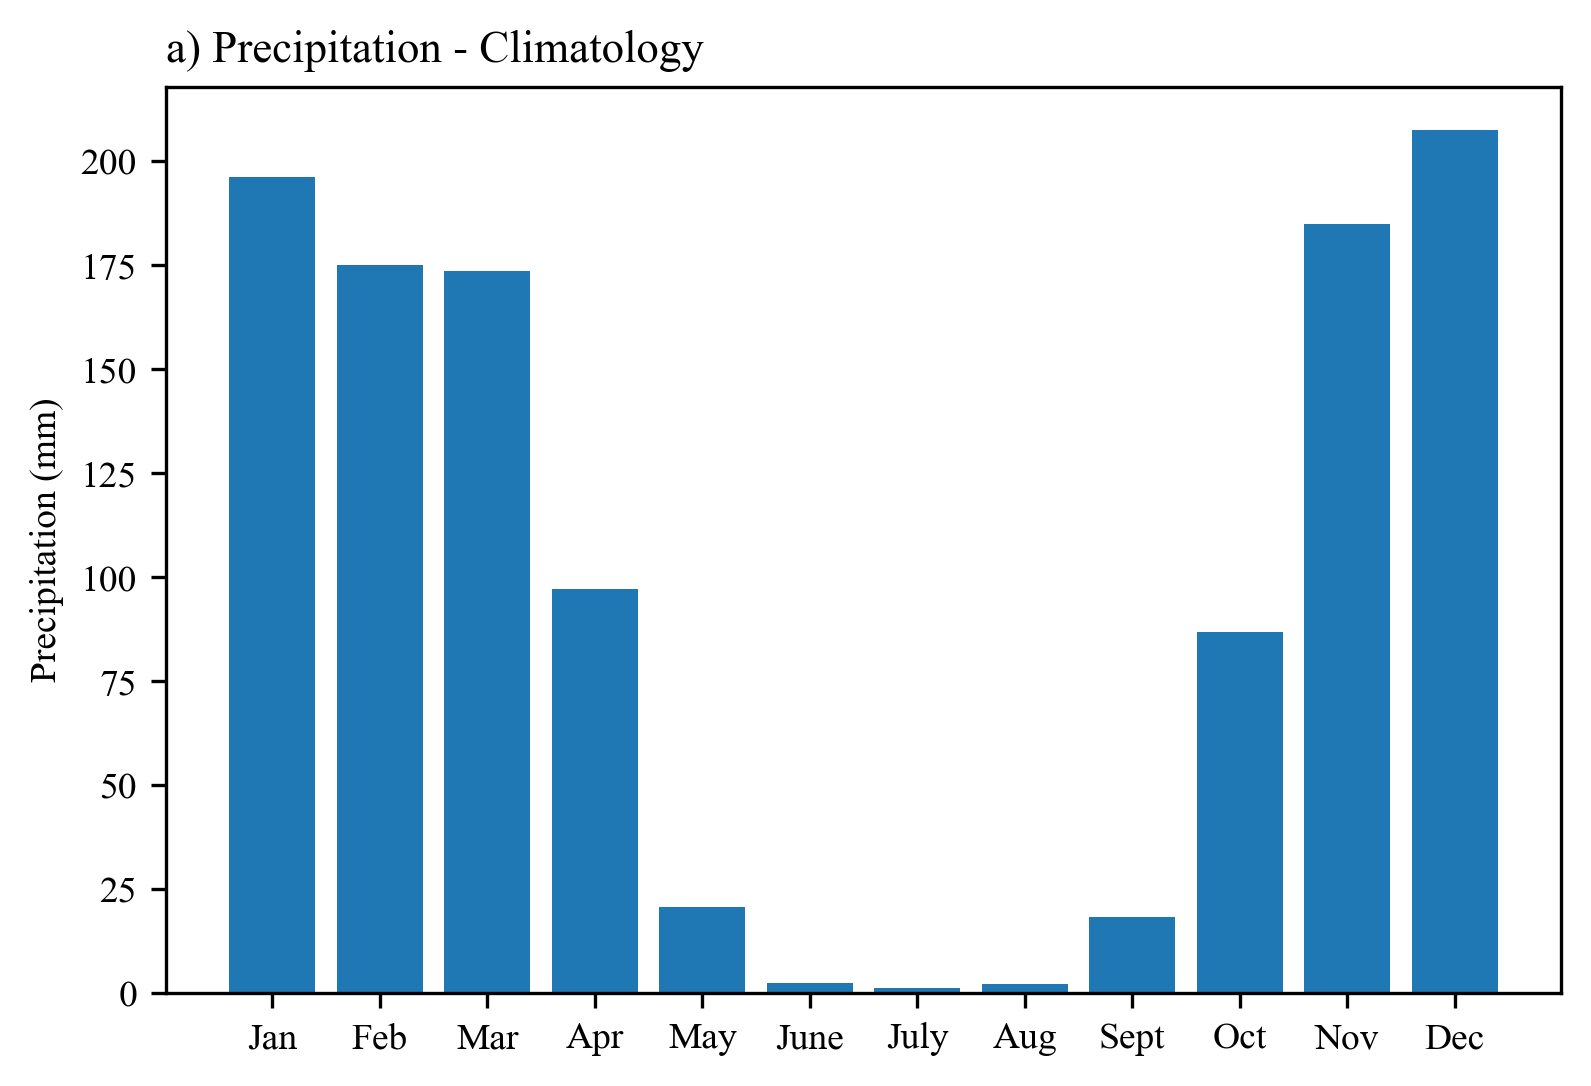
\includegraphics[width = \linewidth]{
                        figs/Pr_Clim.png}
                \end{minipage}
                \hfill    
                \begin{minipage}[t]{0.49\linewidth}
                    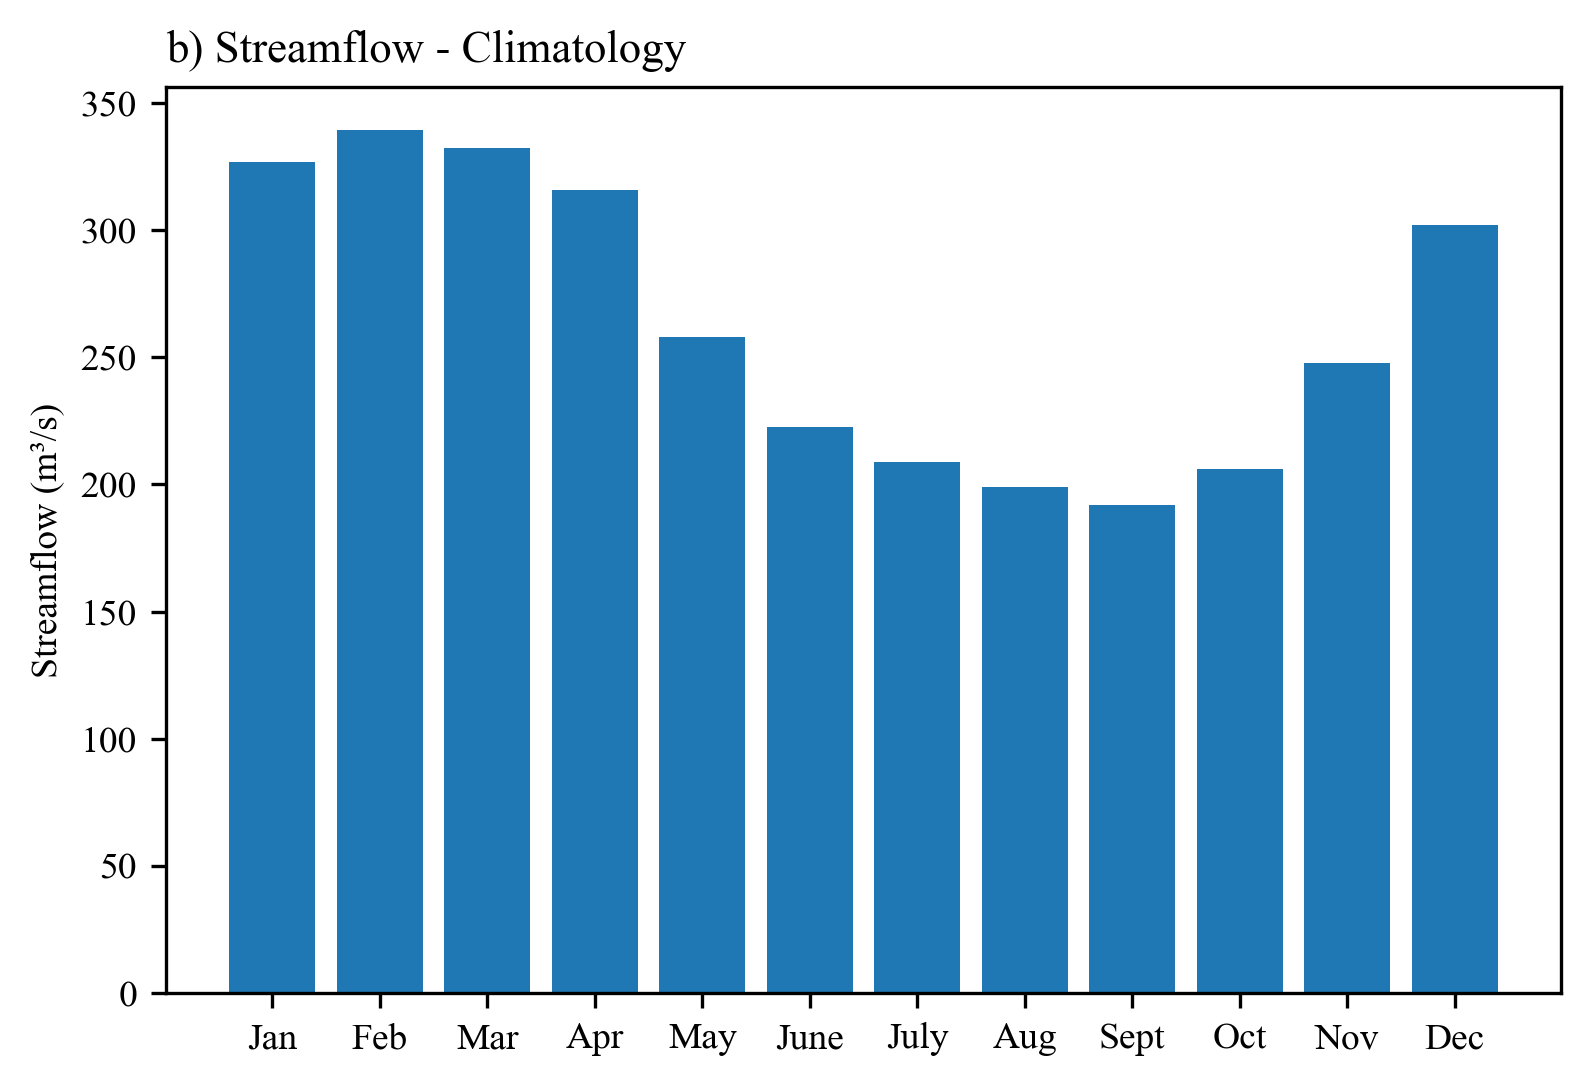
\includegraphics[width = \linewidth]{
                        figs/Vazao_Clim.png}
                \end{minipage}
                
            \caption{
                Climatology of the a) Precipitation and b) Streamflow for the drainage area of  stream gauge 46902000 based on observed data from 1934 to 2020.
            }
            \label{fig:Clima}
        \end{figure*}

    \subsection{Used Data}      
        \subsubsection{Hydrometeorological Data}
            In the present study, hydrometeorological data of precipitation and streamflow were used. The streamflow data were obtained from the measured data at the stream gauge highlighted in the Figure (ID 46902000), available in the National Water Agency's (ANA, from portuguese Agência Nacional de Águas) HIDROWEB database. The daily streamflow time series obtained for this station showed few daily gaps in each of the observed months, making it possible to adopt an uninterrupted period between 1935 and 2020 (86 years).
    
            In relation to precipitation data, the rain gauge stations within and in the vicinity of the drainage area of the 46902000 stream gauge had long gaps and/or considerably short series relative to the size of the available flow series. In order to not exclude streamflow data to enable the use of the above-mentioned observed precipitation information, it was chosen to use the Global Precipitation Climatology Centre (GPCC) monthly precipitation estimates for the entire land surface, getting the data for the period from 1935 to 2020
    
            In this study, we use monthly precipitation totals from the GPCC Full Data Monthly Product Version 2022 provided on a regular grid with a spatial resolution of 1° (longitude and latitude). This product is based on approximately 86,000 stations with almost 10 years of records, providing a regular grid of monthly precipitation totals from 1891 to 2022 at various spatial resolutions: 0.25°, 0.5°, 1.0°, and 2.5°\citep{GPCC:2022}. 
    
            The average precipitation of the basin was obtained by the arithmetic mean between the grid points contained in the rectangle formed by the its maximum and minimum latitudes and longitudes.
        \subsubsection{Land Use and Land Cover Data}
    \blindtext
    
    \subsection{Drought Index}
        In the present study, hydrological and meteorological droughts were characterized by the Standard Precipitation Index (SPI) \citep{mckee1993} and the Standard Runoff Index (SRI) \citep{Shukla2008}, respectively.

        The SPI consists in a comparison between of the accumulated precipitaiton in \textit{n}-month window (scale) with the Cumulative Distribution Function (CDF) of the long-term time series of accumulated precipitation in the same scale. The procedures for its determination can be summarized in three steps: i) determining the CDF of the long-term time series of accumulated precipitation in a \textit{n}-month; ii) determine the probabilities of non-exceedence of the values of this time series and iii) apply these probabilities in the inverse function of a standard normal distribution, returning the SPI \citep{mckee1993, Mishra2007}. 
        
        The determination of the SRI, in turn, adopts the same procedures aforementioned for the determination of the SPI, however, considering the streamflow time series as input data \citep{Shukla2008}. Thus, both indexes, SPI and SRI, can be interpreted as the number of standard deviations of a specific value in a time series in relation to its long-term mean.

        In this study, a 12-month scale (\textit{n} = 12) was adopted for both SPI and SRI. After determining the monthly time series of SPI-12 and SRI-12 from 1935 to 2020, the last month (December) of each year of the time series was adopted, resulting in the annual time series of these indexes. The use of the annual series eliminates the dependence between two consecutive values of the monthly series. As pointed by \citet{Estacio2022}, the SPI-12 monthly time series has a dependency between two consecutive values, because they would differ by only 1 of the 12 values that are accumulated to determine the index on this scale.

        The gamma CDF was adopted to fit the aggregated time series of precipitation and streamflow and to determine the probabilities of non-exceedence of their values. The good fit of this distribution to the used data can be seen in the Quantile-Quantile plot (Q-Q plot) presented in Figure \ref{fig:probplot}. The Q-Q plot shows determination coefficients (\(R^2\)) greater than or equal to 0.99 between the observed quantiles, from the aggregated 12-month time series, and the theoretical quantiles, from the CDF gamma fitted to these time series.

        \begin{figure*}
            \centering
                \begin{minipage}[t]{0.49\linewidth}
                    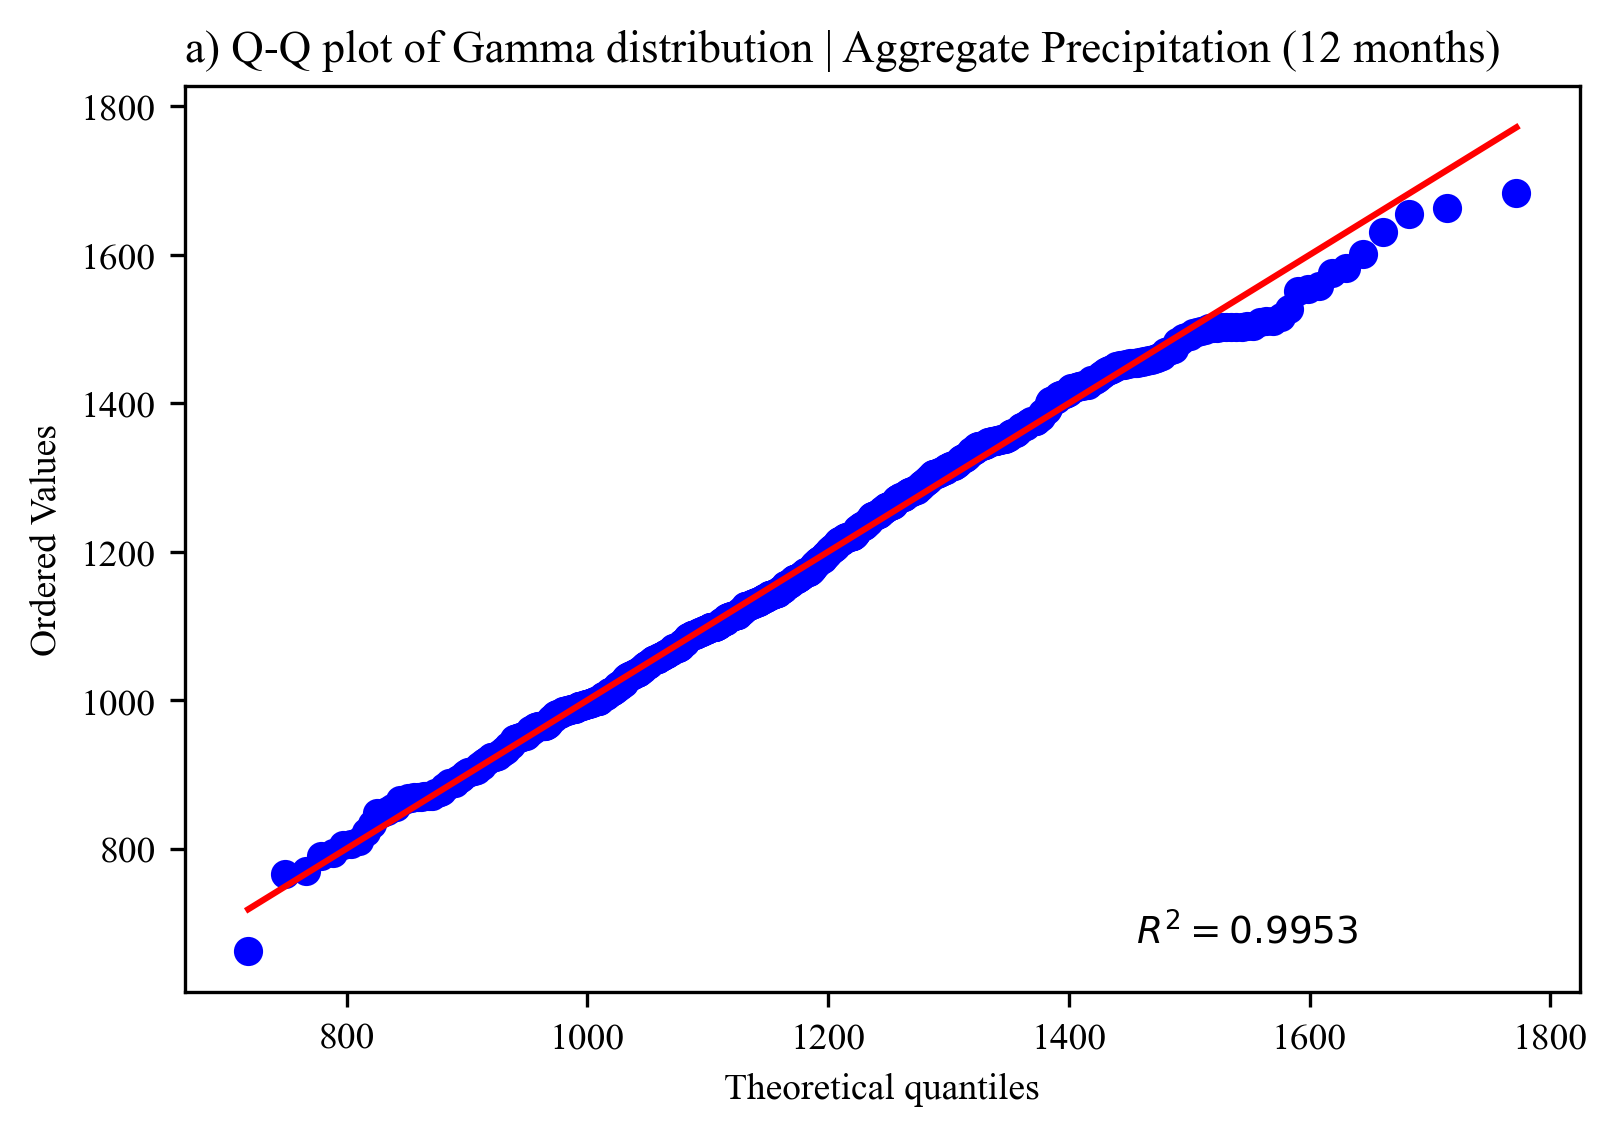
\includegraphics[width = \linewidth]{
                    figs/Q-Q_Plot_Gamma_Pr-12.png}
                \end{minipage}
                \hfill    
                \begin{minipage}[t]{0.49\linewidth}
                    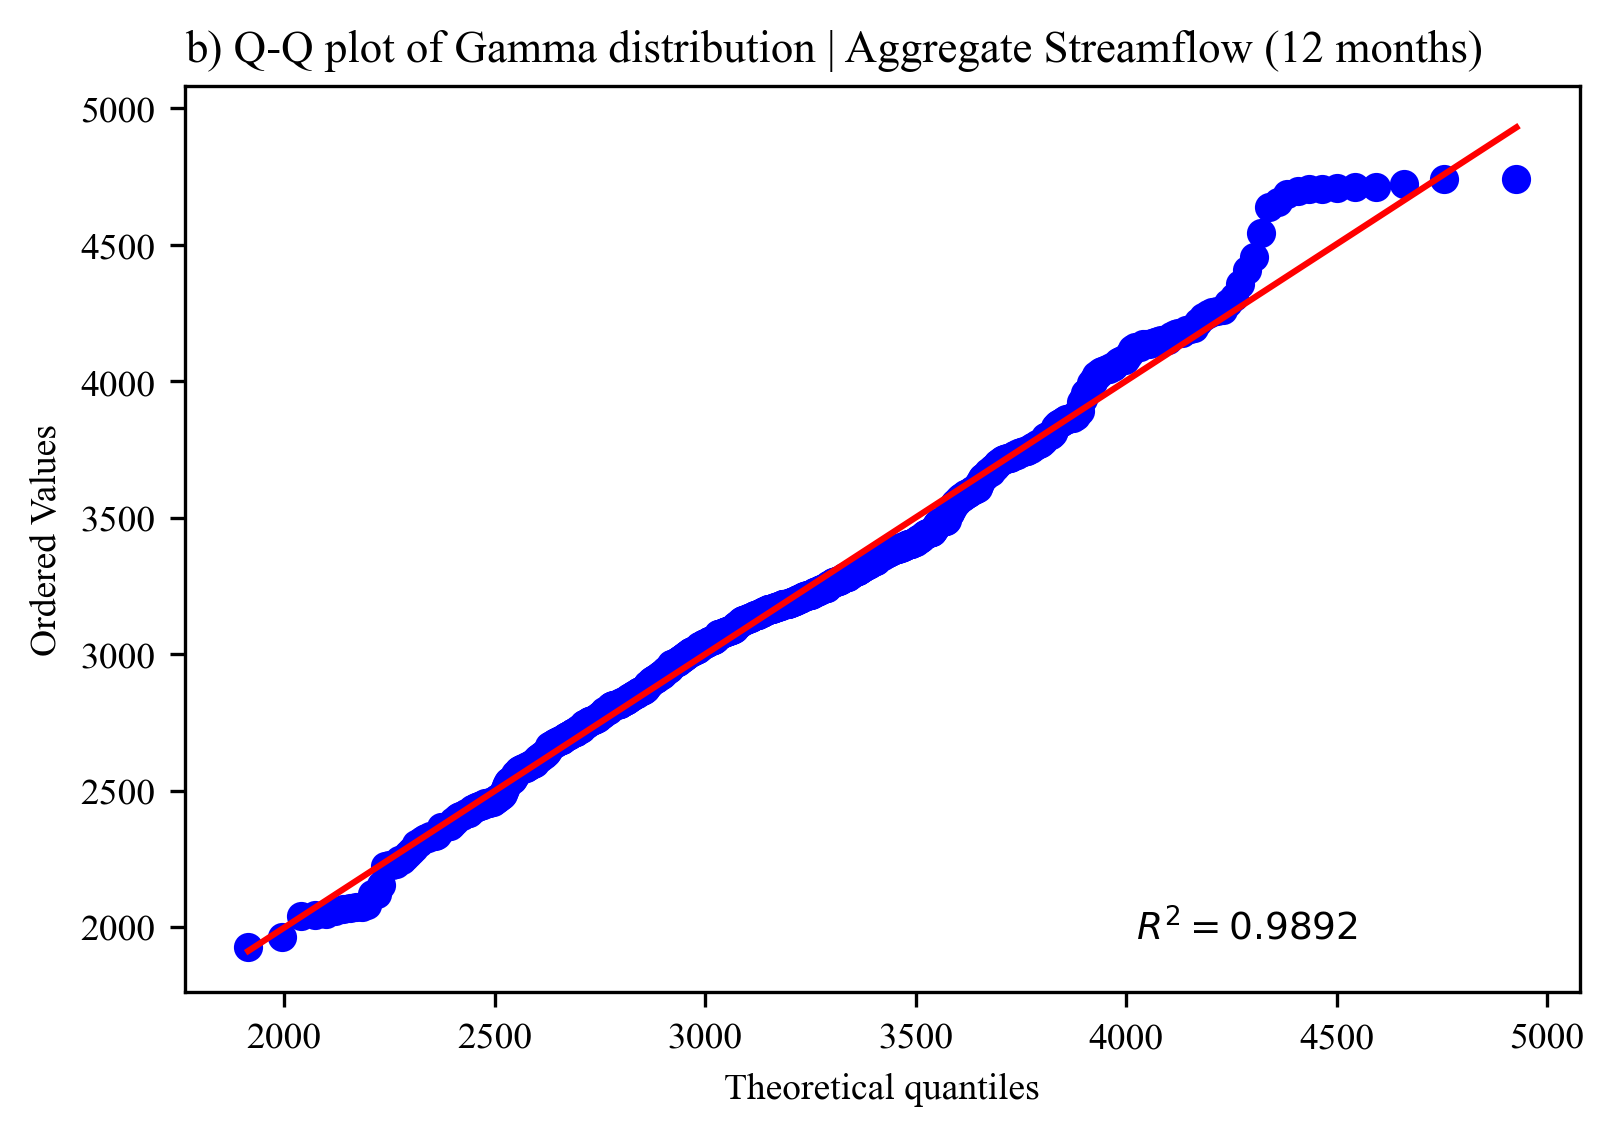
\includegraphics[width = \linewidth]{
                    figs/Q-Q_Plot_Gamma_Q-12.png}
                \end{minipage}            
            \caption{
                Q-Q plot of Gamma distribution for the aggregated a) precipitation and b) streamflow series on a 12-month scale from 1935 to 2020
            }
            \label{fig:probplot}
        \end{figure*}
        
        The density function of a continuous random variable \(x\) that has a Gamma Distribution is given in the Equation \ref{Gamma_pdf}:
        
        \begin{equation}
            f(x) = \frac{({\lambda}x)^{\alpha}}{\Gamma(\alpha)}e^{-{\lambda}x}\frac{1}{x} = \frac{{\lambda}^{\alpha}}{\Gamma(\alpha)}x^{{\alpha}-1}e^{-{\lambda}x}
            \label{Gamma_pdf}
        \end{equation}

        where: $\lambda$ is the rate parameter, $\alpha$ is the shape parameter and $\Gamma(\alpha)$ is the Gamma Function, defined in Equation \ref{Gamma_fun}:

        \begin{equation}
            \Gamma(\alpha) = \int_{0}^{\infty}x^{\alpha}e^{-x}\frac{dx}{x}
            \label{Gamma_fun}
        \end{equation}

        $\Gamma(\alpha)$ and therefore $f(x)$ are defined for \({\forall}x,{\forall}\alpha, {\forall}\lambda > 0\), with \(x, {\alpha}, {\lambda} \in \Re\) \citep{Blitzstein2014}.

        As mentioned by \citet{Estacio2022}, due to the non-definition of the Gamma distribution for $x = 0$, a correction must be made to the non-exceedance probabilities obtained from the CDF Gamma. However, as well as \citet{Estacio2022}, this correction was not performed in this study, because it is completely unlikely that the aggregate precipitation over the year is equal to zero
        

        
    \subsection{Markov Chain}
    
        A Markov chain can be defined as a sequence of random variables contained in a vector \(\vec{X} = [X_{0}, X_{1}, \dots, X_{n}]\) that take on values from a state vector \(\vec{s} = [s_{1}, s_{2}, \dots, s_{k}]\) and following the relation expressed in Equation \ref{markov_prop}, for $n\geq0$
        
        \begin{equation}
            \resizebox{\linewidth}{!}

                {P(X_{n+1} = j|X_{n}=i_{n}, X_{n-1}=i_{n-1}, \dots, X_{0}=i_{0}) = P(X_{n+1} = j|X_{n} = i_{n})
            
                \label{markov_prop}
        \end{equation}
    
        The Equation \ref{markov_prop} expresses the Markov property. This property defines that only the current state is needed to predict the future state \citep{Blitzstein2014,Estacio2022, Mishra2007}. This statement is expressed in the conditional probability \(P(X_{n+1} = j|X_{n}=i_{n})\), i.e., the probability of observing state $j$ at step $n+1$, given the occurrence of state $i$ at step $n$, with $i,j \in \vec{s}$
    
        The behavior of the Markov chain is described by the probabilities of the states contained in the vector $\vec{s}$ moving to any of the other states contained in that vector, including remaining in the initial state. As pointed by \citet{Mishra2007}, these probabilities, also called Transition Probabilities, can be calculated based on the class transitions over the observed data, as shown in Equation \ref{t_prob}.
    
        \begin{equation}
            p_{ij}=P(X_{n+1}=j|X_{n}=i_{n})\approx\frac{n_{ij}}{\sum_{j=1}^{k}n_{ij}}
            \label{t_prob}
        \end{equation}
    
        where: $n_{ij}$ is the transitions occurring for the state $j$ at $n+1$, given the occurrence of the state $i$ at $n$; $\sum_{j=1}^{k}n_{ij}$ is the number of occurrences of the state $i$, regardless of the transition occurred.
    
        The probabilities of all possible transitions can be assembled into a matrix: the Transition Matrix $\tilde{M}$. Since the state vector $\vec{s}$ has dimension $(1xk)$, the matrix $\tilde{M}$ will be a square matrix $(kxk)$, as given in Equation \ref{tb:matrix_T}. The values of $p_{ij}$ are non-negative and the sum of each row of the $\tilde{M}$ must be equal to 1.
    
        \begin{equation}
            \tilde{M} = [p_{ij}]_{kxk} = \begin{bmatrix}
                p_{11} & p_{12} & \dots & p_{1k}\\
                p_{21} & p_{22} & \dots & p_{2k}\\
                \vdots & \vdots & \dots & \vdots\\
                p_{k1} & p_{k2} & \dots & p_{kk}
            \end{bmatrix}
            \label{tb:matrix_T}
        \end{equation}
        
        Another important property of the Markov chain is the stationary distribution of $\vec{X}$. Given a vector $\vec{q}_{0} = [q_{1}, q_{2}, \dots, q_{k}]$, with $q_{i} = P(X_{0}=i)$, representing the probabilities of the $k$ possible states of $\vec{s}$ occur at step 0 of the chain, thus $\vec{q}_{0}$ is the marginal distribution of $X_{0}$. The marginal distribution of $X_{1}$, step 1 of the chain, can be obtained by the multiplication $\vec{q}_{0} \times \tilde{M}$. The marginal distributions for the remaining steps $(X_{2}, X_{3}, \dots,X_{d})$ of the chain can be obtained following the same logic, as shown in Equation \ref{stat_distr}:    
    
        \begin{equation}
            \vec{q}_{2} = \vec{q}_{1}\times\tilde{M} = \vec{q}_{0}\times\tilde{M^{2}}, \dots, \vec{q}_{d} =  \vec{q}_{0}\times\tilde{M^{d}}
            \label{stat_distr}
        \end{equation}
    
        Over long run, i.e., for large values of $d$, a convergence of the marginal distributions is reached $(\vec{q}_{d} = \vec{q}_{d+1} = \vec{q}_{d+2})$, therefore $\vec{q}_{d}$ is defined as the stationary distribution of $\vec{X}$. In other words, stationary distribution represents the marginal distribution of an initial state, in which any transition performed will result in a final state with the same marginal distribution as the initial state:  $\vec{q}_{d+1}=\vec{q}_{d}\times\tilde{M}|\vec{q}_{d+1}=\vec{q}_{d}$ \citep{Blitzstein2014}.
    
    \subsection{Drought State Transitions}

        In order to assess the impact of anthropic changes on the drought class transitions, the entire SPI and SRI periods are divided into two sub-periods: pre- and post-anthropic changes periods.
    
        As pointed by \citet{Pimentel2022}, the soybean production in the west of the Brazilian state of Bahia, where the analyzed basin is located, showed a strong growth trend starting in 1985, rapidly increasing its percentage of participation in Brazilian soy production between 1985 and 1995. In 2005, this region was already responsible for 4.50\% of the Brazilian soy production.
    
        According to the above-metioned information, it was decided to divide the annual time series of SPI-12 and SRI-12 (1935-2020) into the pre-anthropic change period (P1), from 1935 to 1984 (49 years), and the post-anthropic change period (P2), from 1985 to 2020 (36 years).

        To determine the transitions between the drought classes, the continuous values of the SPI and SRI time series in both periods were converted into drought classes. For this conversion, the classification presented by \citet{mckee1993} was adapted. This adapted classification was similar to the one adopted by \citet{Estacio2022}. 
        
        The Table \ref{tb:drought_class} shows the drought classes adopted in this study and compares it with the classification presented by \citet{mckee1993}. The Severe and Extreme Drought classes were aggregated into a single class: Severe or Extreme Drought (SED). Extreme Drought events have a low probability of occurrence, therefore, it is plausible that this event occurs in only one of the analyzed periods. In order to standardize the possible transition states in periods P1 and P2 and, consequently, their transition matrices, it was decided to group these two drought classes.

        With the continuous SPI-12 and SRI-12 values converted into drought classes (Table \ref{tb:drought_class}), the transitions matrices were determined with Equation \ref{t_prob}. Four transition matrices were determined: i) SPI-12 in P1 periods, ii) SPI-12 in P2 period, iii) SRI-12 in P1 period and iv) SRI-12 in P2 period. These transition matrices were used to determine the stationary distribution of each respective Markov chain with the procedure presented in Equation \ref{stat_distr}.

        
        \begin{table*}[pos=h]
            \caption{
                Adopted drought classes for meteorological (SPI) and hydrological (SRI) droughts
                }
            \label{tb:drought_class}
            \begin{tabular*}{\tblwidth}{@{\extracolsep{\fill}} c c c}
                \toprule
                    Index Value & \citet{mckee1993} & Adopted drought classes\\
                \midrule
                    $SPI, SRI \geq 0$ & No Drought & No Drought (ND)\\
                    $-1.0 < SPI,SRI < 0$ & mild Drought & mild Drought (mD) \\
                    $-1.5 < SPI,SRI \leq -1.0$ & Moderate Drought & Moderate Drought (MD) \\
                    $-2.0 < SPI,SRI \leq -1.5$ & Severe Drought & \multirow{2}{*}{Severe or Extreme Drought (SED)}\\
                    $SPI,SRI \leq -2.0$ & Extreme Drought & \\
                \bottomrule
                \footnotesize Source: adapted from \citet{mckee1993, Estacio2022}
                \end{tabular*}
            \end{table*}
        
    \subsection{Minimum Reference Streamflow}
        Minimum Reference Streamflows (MRS) are important metrics for water resources management and planning, as they provide information about the basin's water availability. 
        
        In this study, the MRS were used to evaluate the basin's water availability throughout the evaluated period, seeking to establish relationships between its behavior and the anthropic modifications induced in the analyzed basin.
        
        For this purpose, the entire period (1935 - 2020) gave rise to six subperiods, as presented in Table \ref{tb:sub_periods_min_flow}. This subdivision was arbitrary, however it was attempted to standardize the duration of each subperiod and the year 1985 was considered as the reference point for defining the periods of pre- and post anthropic change, as well as in the analysis of drought state transitions

        \begin{table}[width=.9\linewidth, cols=5, pos=h]
            \caption{
            Subperiods considered for analysis of the minimum reference streamflow
            }
            \label{tb:sub_periods_min_flow}
            \begin{tabular*}{\tblwidth}{@{\extracolsep{\fill}} c c c}
            \toprule
                Subperiod & Interval & Anthropic Change\\
            \midrule
                SP1 & 1935 - 1954 (20 yrs) & Pre-Change \\
                SP2 & 1955 - 1969 (15 yrs) & Pre-Change \\
                SP3 & 1970 - 1984 (15 yrs) & Pre-Change \\
                SP4 & 1985 - 2000 (16 yrs) & Post-Change \\
                SP5 & 2001 - 2010 (10 yrs) & Post-Change \\
                SP6 & 2011 - 2020 (10 yrs) & Post-Change \\
            \bottomrule
            \end{tabular*}
        \end{table}

        Two MRS were adopted: $Q_{95}$ and $Q_{7,10}$, determined for each subperiod in Table \ref{tb:sub_periods_min_flow}. In addition, a trend analysis was performed on the annual minimum daily streamflow time serie from 1935 to 2020 using the non-parametric Mann-Kendall test and the Sen's slope. More information about the Mann-Kendall test and Sen's slope (MKS) can be found at \citet{Lima2022}

        The $Q_{95}$ represents the streamflow associated with a exceedence probability of 95\%, i.e, this streamflow remains in the watercourse at least 95\% of the time \citep{Abreu2022}. In order to determine it, the Flow-Duration Curves (FDC) for each subperiod were determined. The FDC's determination considered all daily observations of each subperiod, without moving averages to eliminate day-to-day variations.

        The FDC establishes the relationship between the streamflows and their exceedance probability, i.e., the percentage of time that this flow is exceeded or equaled in the entire reference period used in its determination. The excedeence probability is the complement of the non-excedeence probability, thus the FDC can be determined with the CDF of the used data \citep{Abreu2022, Verma2016}.

        In this study, the FDC for each subperiod were determined empirically with the percentiles of their daily streamflow time series. Percentiles divide a data sample, sorted in ascending order, into 100 parts. For each of these parts, a non-exceedance probability can be associated such that the $n$-percentile has $n\%$ of non-exceedance probability. In this way, the exceedance probabilities and, consequently, the FDC curve can be determined with the complement of the non-exceedance probabilities of percentiles of the daily streamflow data for each subperiod.

        The $Q_{7,10}$, in turn, indicates the minimum 7-day moving average annual of streamflow associated with a 10-year recurrence period, i.e., it is expected that this average streamflow will be exceeded on average of 9 out every 10 years. \citep{Reilly2003}. For its determination, the following four steps were adopted: i) determination of 7-day moving average of daily streamflow time serie; ii) selection of the minimum value of this moving average for each year, giving rise to a time series of annual minima; iii) fitting this time series of annual minima to a CDF, in this study, the Left-Skewed CDF Gumbel was adopted and iv) Obtaining the $Q_{7,10}$ with the Left-Skewed CDF Gumbel inverse function, considering a non-exceedance probability of 0.1\%, i.e., a 10-year recurrence period.

    

%\section{Results}
    \subsection{Changes in Land Use and Land Cover}
    \subsection{Drought State Transitions}
    	The Table \ref{tb:abs_freq_drought_class}  presents the relative frequency of each meteorological (SPI-12) and hydrological (SRI-12) drought class for the periods P1 and P2. In P1 period, it can be observed that the most recurrent drought classes are ND and mD for both SPI-12 and SRI-12. Between periods P1 and P2, similar changes in relative frequencies are observed for both drought indexes, they are: reductions in the relative frequencies of drought classes ND, mD and MD and an increase in the relative frequency of class SED.
    	
    	In period P2, the drought class ND remains the one with the highest relative frequency for both SPI-12 and SRI-12. For SPI-12, there is an increase of 11.44\% in the relative frequency of the SED class and a decrease of 8.56\% in the mD class between P1 and P2, equalizing the relative frequency of these two classes in P2. For SRI-12, the changes in relative frequencies for SED and mD classes between P1 and P2 periods are, respectively, $+14.67\%$ and $-8.22\%$. Despite these changes in relative frequencies, ND and mD classes of SRI-12 are still the most recurrent in the P2 period.
    	 
		\begin{table}[width=.9\linewidth, cols=5]
            \caption{
            Relative Frequencies of SPI and SRI drought classes in P1 (50 yrs) and P2 (36 yrs) periods.
            }
            \label{tb:abs_freq_drought_class}
             \begin{tabular*}{\tblwidth}{@{\extracolsep{\fill}} c| c c c c}
            \toprule
                  & ND & mD & MD & SED & Duration\\
            \midrule
                SPI-12 (P1) & 50.00\% & 28.00\% & 14.00\% & 8.00\% \\
                SPI-12 (P2) & 47.22\% & 19.44\% & 13.89\% & 19.44\% \\
                SRI-12 (P1) & 56.00\% & 36.00\% & 6.00\% & 2.00\% \\
                SRI-12 (P2) & 50.00\% & 27.78\% & 5.56\% & 16.67\% \\
            \bottomrule
            \end{tabular*}
        \end{table}  
  
        The Figure \ref{fig:t_probs} shows the transition matrices of the meteorological and hydrological droughts classes for both P1 and P2 periods.
        
        Regarding the changes in the transition probabilities of hydrological droughts (SRI-12), significant changes can be observed given the occurrence of both SED and MD drought classes. For the occurrence of the SED drought class, the transition probabilities in period P2 are 66.67\% to remain in the SED class and 16.67\% to regress to the MD or md drought classes; in period P1, the unique possible transition, i.e. 100\% probability, is to regress to a MD drought class.

        In relation to MD drought class occurrence, two equiprobable transitions are observed in period P2: progress to SED drought class or regress to mD drought class, and three equiprobable transition are seen in period P1: permanence in the MD drought class or regression to the mD or ND drought classes.

        No significant changes were observed in the transition probabilities given the occurrence of the ND or mD classes, however, the possibilities of transition from ND to SED (3.7\%) in the P1 period, which does not occur in the P2 period, and transition from mD to SED (11.11\%) in the P2 period, that does not occur in the P1 period, can be highlighted.

        Concerning the changes in the transition probabilities of meteorological droughts (SPI-12), except for the occurrence of the mD class, no changes were observed in the possible transitions, only in the values of the transition probabilities. 
        
        For an occurrence of mD drought class, one can observe that there are three possibles transitions in P1 period are: regress to ND (35.71\%), permanence in mD class (42.86\%) and progress to MD class (21.43\%). However, in P2 period, these three possibles transition are reduced from two: regress to ND (71.43\%) and progress to SED (28.57\%).

        It is worth noting the changes in the probabilities of the possible transitions between the P1 and P2 periods, given the occurrence of a ND drought class. In P1 period, the most probable transition for this drought class occurrence is to remain in the ND class (52.00\%). In P2 period, two equiprobable transitions appear: permanence in ND class (31.25\%) and progress to SED class (31.25\%). An increase in the probability of progression for MD can also be observed from 12.0\% at P1 to 25.0\% at P2
        
        \begin{figure*}
            \centering
                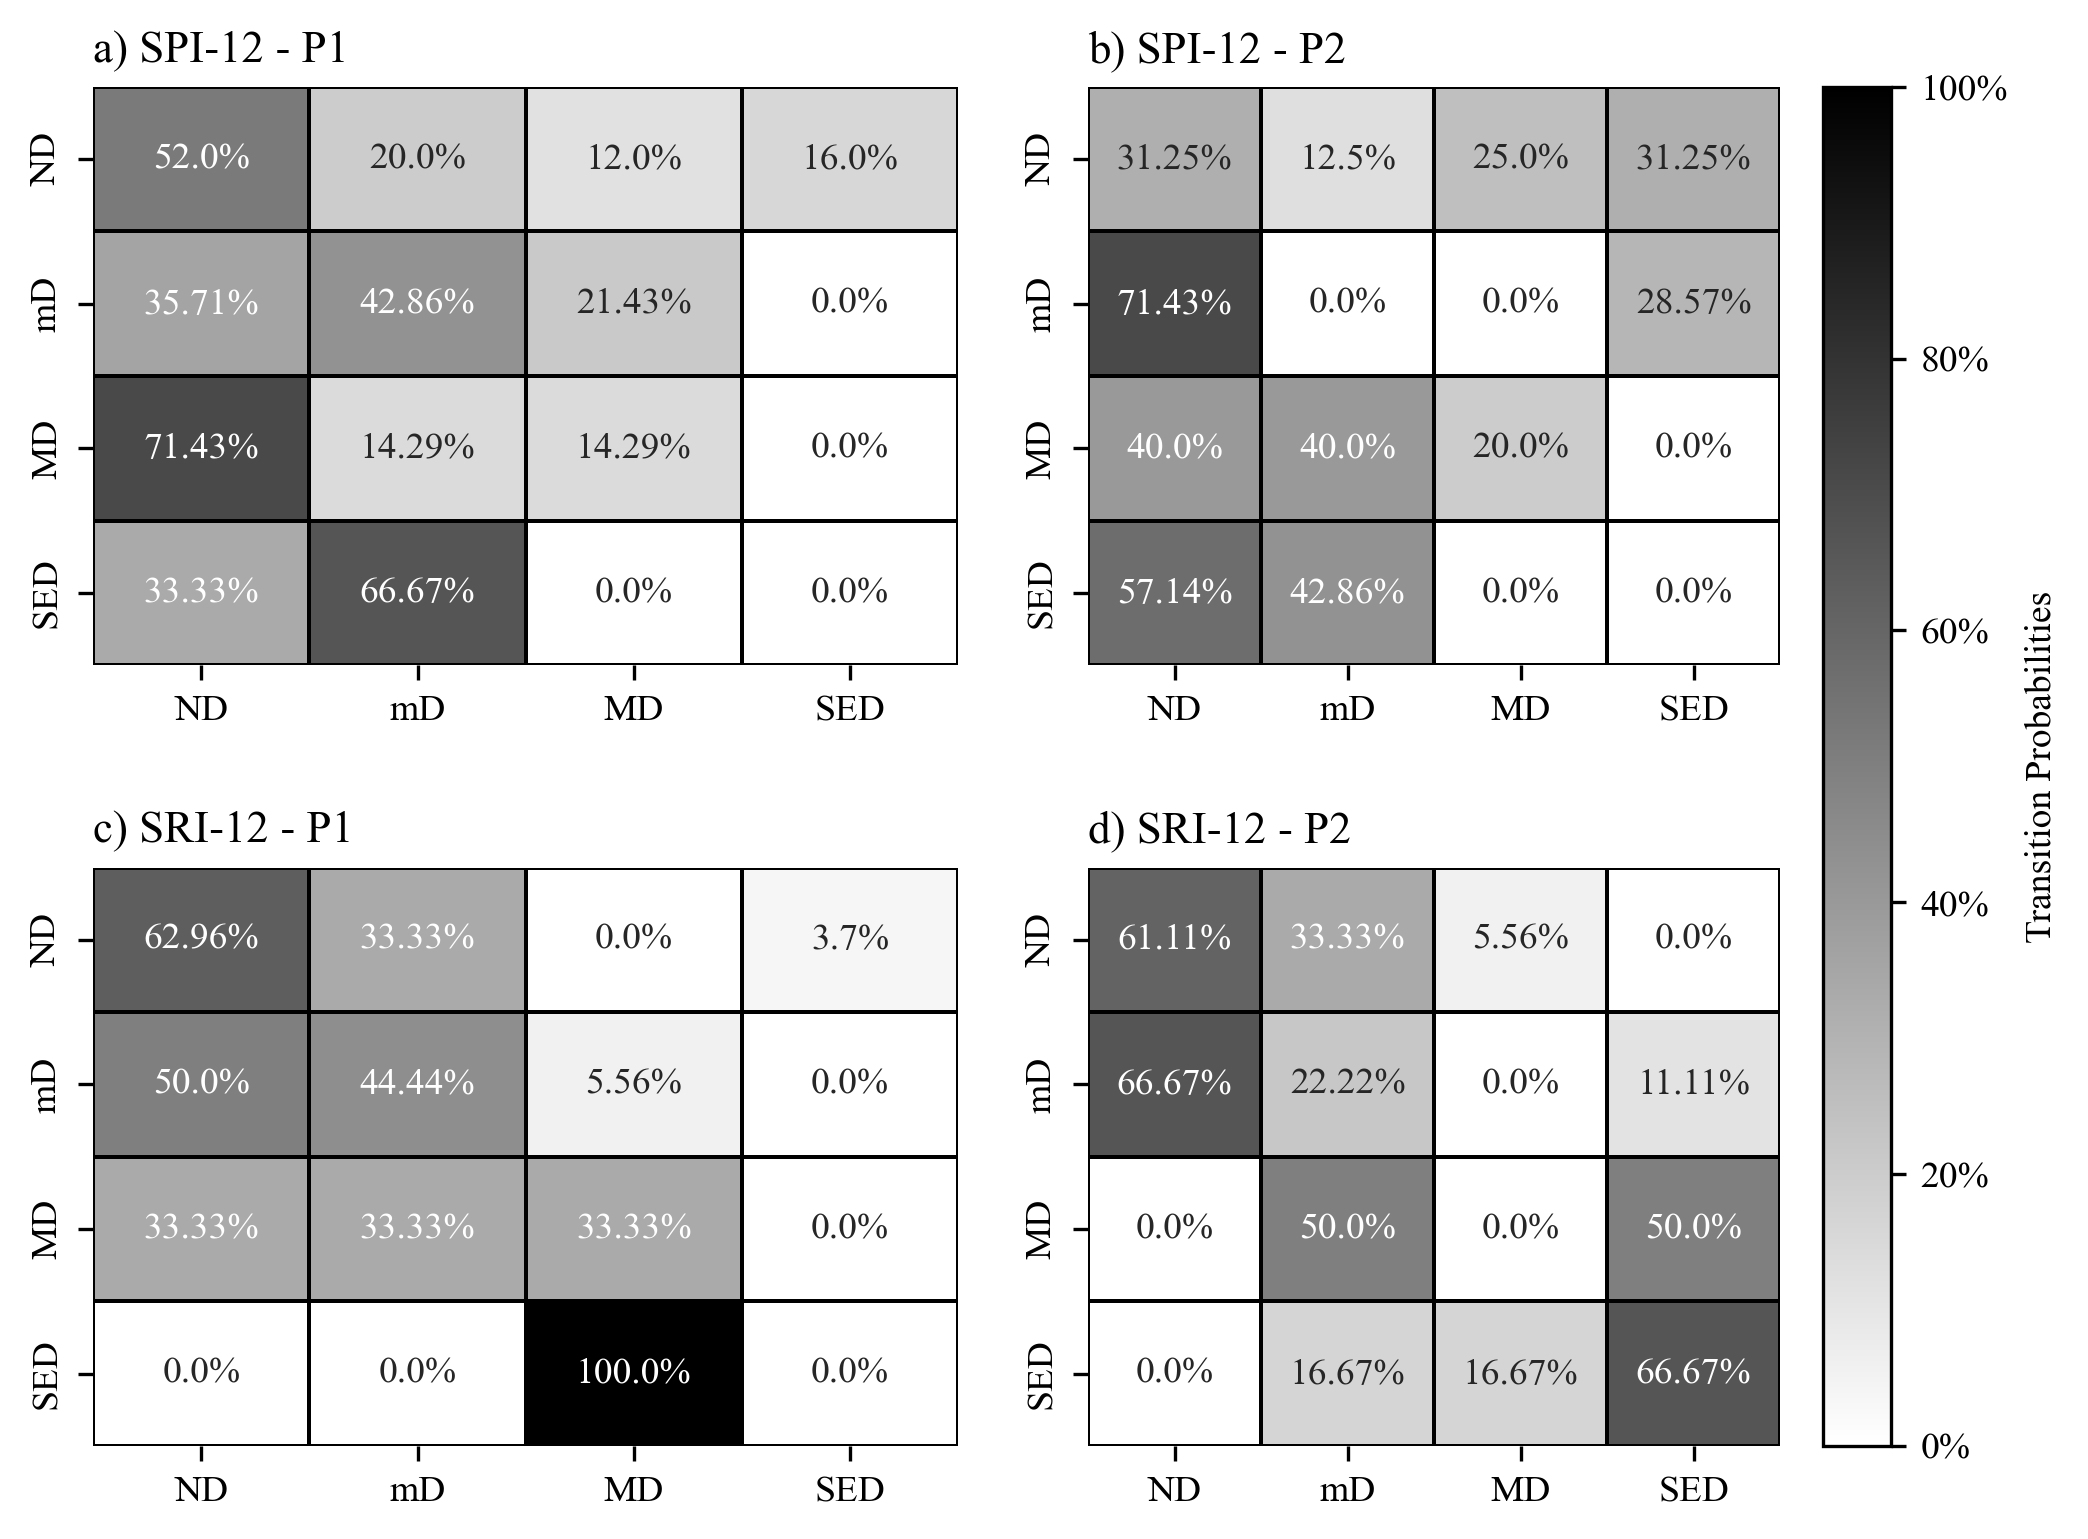
\includegraphics[scale = 1]{
                figs/SPI_SRI_Transition_Matrix.png
                }
            \caption{
                Transition matrices of the adopted drought classes for the following time series: a) SPI-12 in period P1, b) SPI-12 in period P2, c) SRI-12 in period P1 and d) SRI-12 in period P2
            }
            \label{fig:t_probs}
        \end{figure*}
        
        \begin{table}[width=.9\linewidth, cols=5]
            \caption{
            Stationary distribution of the Markov chains constructed for SPI-12 and SRI-12 for both P1 and P2 periods.
            }
            \label{tb:std_distr}
            \begin{tabular*}{\tblwidth}{@{\extracolsep{\fill}} c| c c c c}
            \toprule
                  & ND & mD & MD & SED\\
            \midrule
                SPI-12 (P1) & 48.49\% & 29.57\% & 14.18\% & 7.76\% \\
                SPI-12 (P2) & 45.71\% & 20.00\% & 14.29\% & 20.00\% \\
                SRI-12 (P1) & 55.10\% & 36.73\% & 6.12\% & 2.04\% \\
                SRI-12 (P2) & 48.29\% & 28.17\% & 5.66\% & 17.88\% \\
            \bottomrule
            \end{tabular*}
        \end{table}

     \subsection{Minimum Reference Streamflow}
        The Minimum Annual Daily Streamflow from 1935 to 2020 is presented in the Figure \ref{fig:Q_min}. The MKS method pointed to a decreasing trend between 1935 and 2020. One can observe that this behavior is not predominant throughout the entire period.
        
        \begin{figure*}
            \centering
                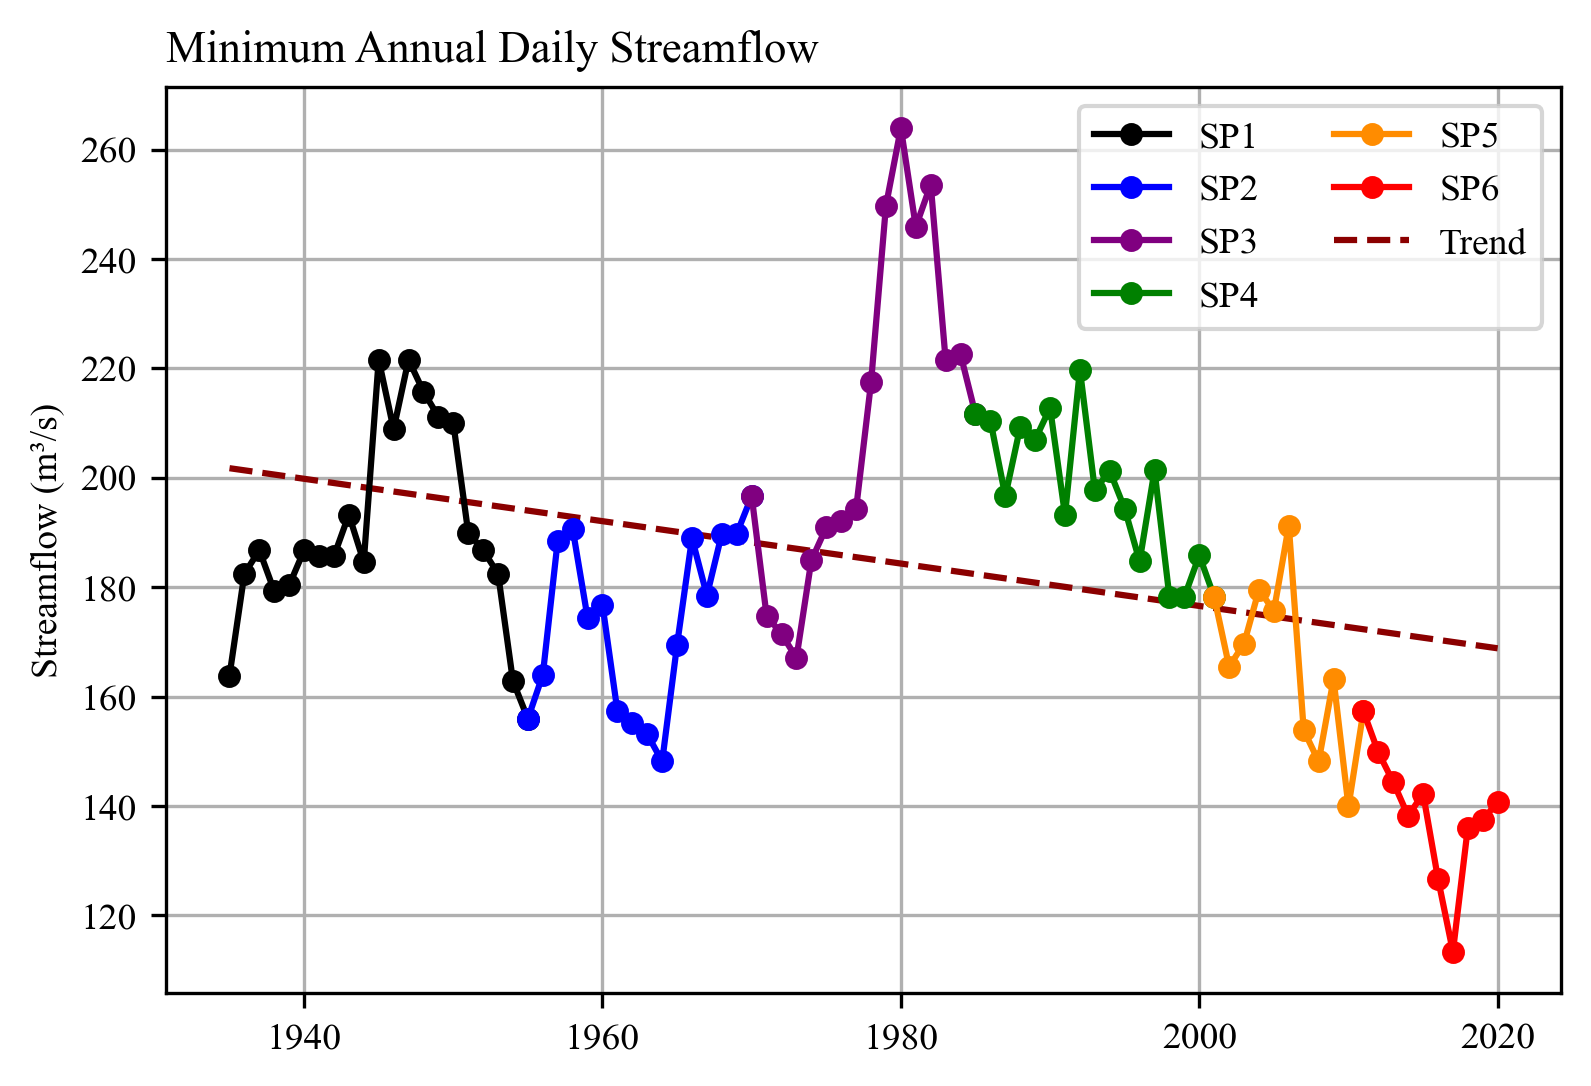
\includegraphics[scale = 1]{
                figs/Q_min_anual.png
                }
            \caption{
                Minimum Annual Daily Streamflow time series from 1935 to 2020. 
            }
            \label{fig:Q_min}
        \end{figure*}
        
        A marked interannual variability can be observed between the subperiods SP1 and SP3. In the subperiod SP3, a strong increasing behavior is noted, reaching the peak of the time series in 1980. 
        
        A predominantly decreasing behavior was observed between SP4 and SP6 periods, reaching the minimum of the time series in 2017. The behavior of these sub-periods attributes to this time series the decreasing trend evidenced by the MKS method.

        The Figure \ref{fig:FDC} and the Table \ref{tb:min_ref_flow} shows, respectively, the FDC curves and the adopted MRS ($Q_{95}$ and $Q_{7,10}$) for each subperiod highlighted in the Table \ref{tb:sub_periods_min_flow}. 

        \begin{figure*}
            \centering
                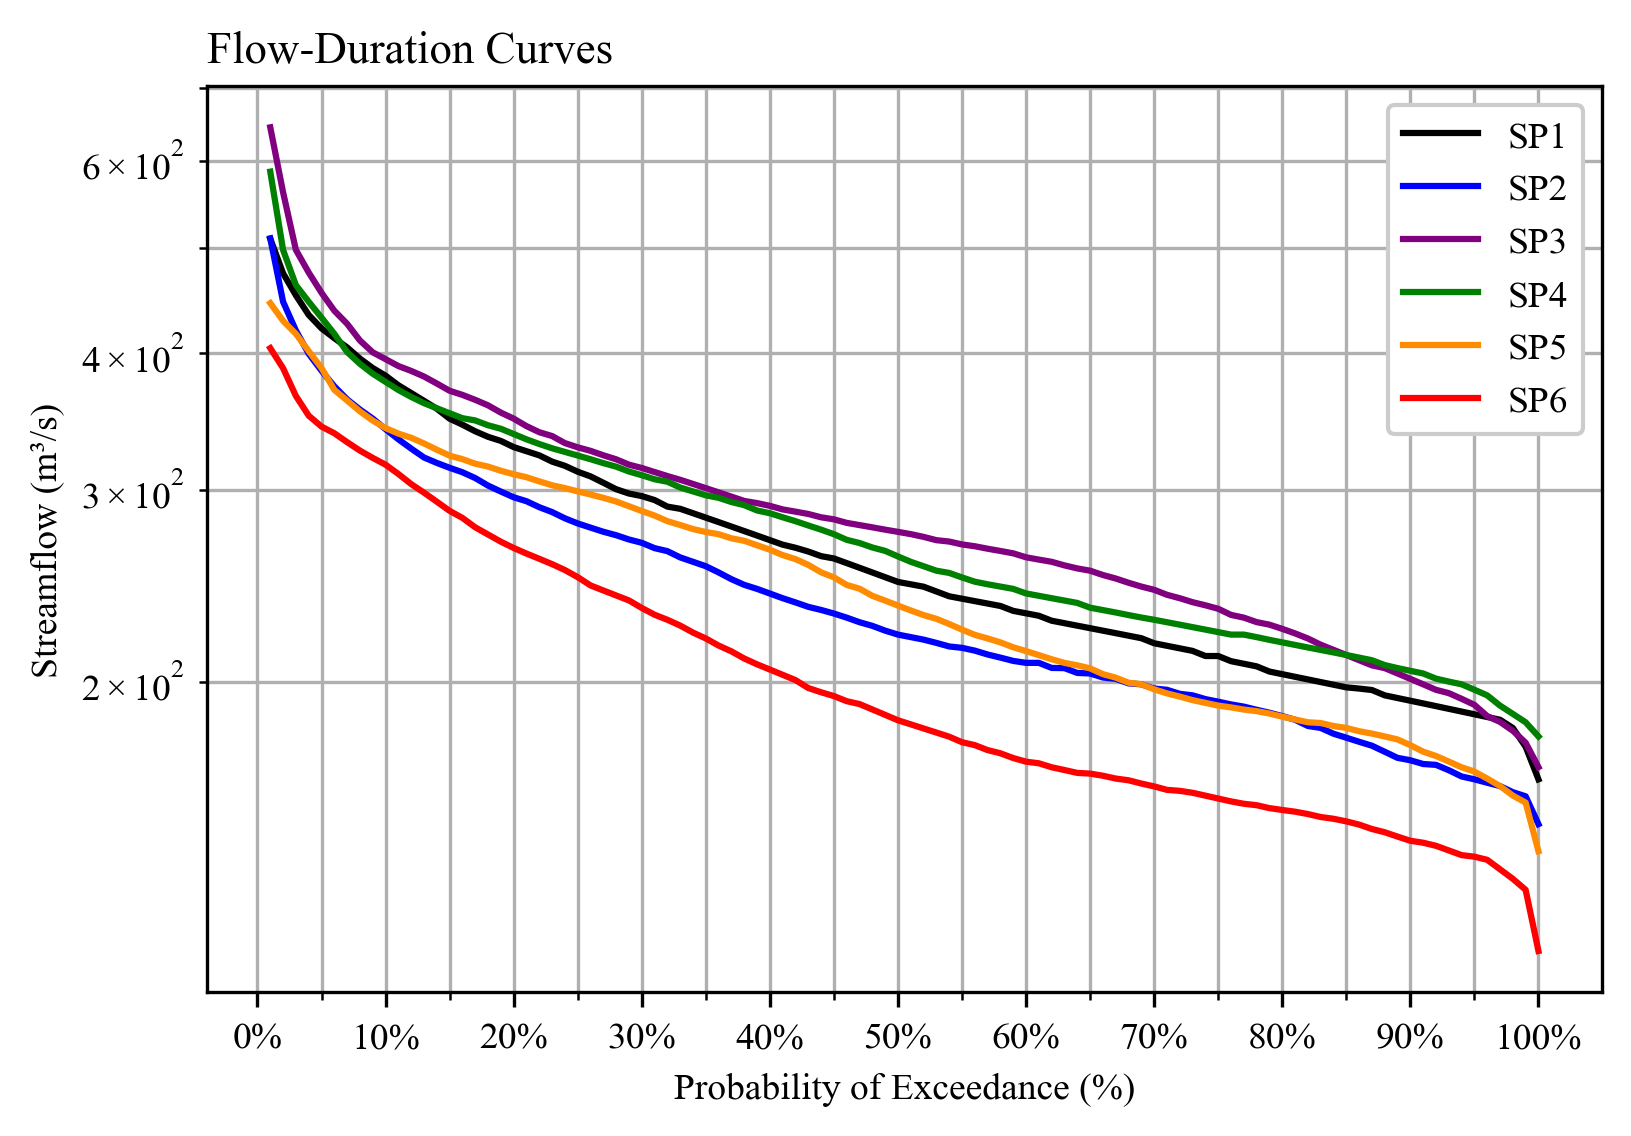
\includegraphics[scale = 1]{
                figs/Curvas_Permanencia.png
                }
            \caption{
                Flow-Duration Curves for each adopted subperiod (Table \ref{tb:sub_periods_min_flow})
            }
            \label{fig:FDC}
        \end{figure*}

        \begin{table}[width=.9\linewidth, cols=5]
            \caption{
            Minimum Reference Streamflows for each adopted subperiod
            }
            \label{tb:min_ref_flow}
            \begin{tabular*}{\tblwidth}{@{\extracolsep{\fill}} c c c}
            \toprule
                Subperiod & $Q_{95}\;(m^{3}/s)$ & $Q_{7,10}\;(m^{3}/s)$\\
            \midrule
                SP1 & 186.75 & 215.55 \\
                SP2 & 162.80 & 190.81 \\
                SP3 & 190.52 & 251.26 \\
                SP4 & 196.68 & 214.87 \\
                SP5 & 165.49 & 185.81 \\
                SP6 & 138.29 & 152.61 \\
            \bottomrule
            \end{tabular*}
        \end{table}

        The predominantly decreasing behavior of the minimum annual daily streamflow after SP3 produces successive reductions in FDC's streamflows in the SP4, SP5 and SP6 subperiods. The SP6 subperiod, according to its FDC, presented the lowest water availability of the entire evaluated period (1935-2020).

        The subperiods SP3 and SP4 show an interesting behavior in their FDC. The SP4's FDC shows the highest streamflow values for almost all exceedance probabilities, however, for large values ($\geq 80\%$), the streamflows of the SP4's FDC surpass of the SP3's FDC. According to the Figure \ref{fig:Q_min}, despite the peak value in SP3, this subperiod presented 8 of 15 years with minimum daily streamflows lower or of the same magnitude as those observed in SP4, which may justify the FDC's behavior above-mentioned.
        
        Regarding $Q_{95}$ , a significant variability in its value is observed between the SP1, SP2 and SP3 subperiods, from 186.75 $m^{3}/s$ to 162.80 $m^{3}/s$ and from 162.80 $m^{3}/s$ to 190.52 $m^{3}/s$. This behavior can be explained by the marked interannual variability of the annual minimum daily flow observed between these subperiods.

        In SP4 there is the highest value of $Q_{95}$  among the subperiods, 196.68 $m^{3}/s$, indicating the subperiod with the highest water availability. However, from this subperiod onwards, successive reductions are observed in the $Q_{95}$ values, reaching the lowest value in SP6: 138.29 $m^{3}/s$, a reduction of almost 30\%.

        Regarding $Q_{7,10}$, a similar behavior to that observed in $Q_{95}$ is noted, except for the occurrence of its highest value in SP3 instead of SP4. After the occurrence of this peak at SP3 (251.26 $m^{3}/s$), successive reductions are observed until reaching its minimum value at SP6 (152.61 $m^{3}/s$), a reduction of approximately 39\%.
        


        

%\section{Discussions}

    The analysis of drought state transitions showed significant changes in hydrological drought state transitions between the P1 and P2 periods that were not observed for meteorological droughts. 
    
    Hydrological droughts, given the occurrence of more severe drought states (MD or SED), presented a higher probability of intensification or permanence of these drought states in the P2 period.


%\section{Conclusions}
    \blindtext
\section{Cross-references}


\appendix
\section{My Appendix}
Appendix sections are coded under \verb+\appendix+.

\verb+\printcredits+ command is used after appendix sections to list 
author credit taxonomy contribution roles tagged using \verb+\credit+ 
in frontmatter.

\printcredits

%% Loading bibliography style file
%\bibliographystyle{model1-num-names}
\bibliographystyle{cas-model2-names}

% Loading bibliography database
\bibliography{refs}


\vskip3pt

% \bio{}
% Author biography without author photo.
% Author biography. Author biography. Author biography.
% Author biography. Author biography. Author biography.
% Author biography. Author biography. Author biography.
% Author biography. Author biography. Author biography.
% Author biography. Author biography. Author biography.
% Author biography. Author biography. Author biography.
% Author biography. Author biography. Author biography.
% Author biography. Author biography. Author biography.
% Author biography. Author biography. Author biography.
% \endbio
%
%% \bio{figs/pic1}
% Author biography with author photo.
% Author biography. Author biography. Author biography.
% Author biography. Author biography. Author biography.
% Author biography. Author biography. Author biography.
% Author biography. Author biography. Author biography.
% Author biography. Author biography. Author biography.
% Author biography. Author biography. Author biography.
% Author biography. Author biography. Author biography.
% Author biography. Author biography. Author biography.
% Author biography. Author biography. Author biography.
% \endbio
%
%% \bio{figs/pic1}
% Author biography with author photo.
% Author biography. Author biography. Author biography.
% Author biography. Author biography. Author biography.
% Author biography. Author biography. Author biography.
% Author biography. Author biography. Author biography.
% \endbio

\end{document}

